\documentclass[preprint,12pt]{elsarticle}

\usepackage{amsmath,amssymb,amsfonts}
\usepackage{algorithm}
\usepackage{algpseudocode}
\usepackage{graphicx}
\usepackage{textcomp}
\usepackage{url}
\usepackage{booktabs}
\usepackage{tabularx}
\usepackage{bm}
\usepackage{hyperref}
\usepackage{lineno}

\hypersetup{
    colorlinks=true,
    linkcolor=blue,
    citecolor=blue,
    urlcolor=blue
}

\graphicspath{{figures/}}

\journal{Computers and Electrical Engineering}

\begin{document}

\begin{frontmatter}

\title{Vision-Based 2D Scan Generation for Obstacle Avoidance Using Floor Segmentation}

\author[inst1]{Hyunseo Lee\fnref{fn1}}
\author[inst1]{Gunmin Yoo\fnref{fn1}}
\author[inst1]{Hyunwoo Gu\fnref{fn1}}
\author[inst1]{Sung Soo Hwang\corref{cor1}}
\ead{sshwang@handong.edu}

\fntext[fn1]{Hyunseo Lee, Gunmin Yoo, and Hyunwoo Gu contributed equally to this work.}
\cortext[cor1]{Corresponding author.}

\affiliation[inst1]{organization={School of Artificial Intelligence, Computer and Electrical Engineering, Handong Global University},
            city={Pohang},
            postcode={37554},
            state={Gyeongsangbuk-do},
            country={Republic of Korea}}

\begin{abstract}
Autonomous mobile robots (AMRs) operating in structured indoor environments typically rely on planar LiDAR sensors for real-time obstacle avoidance. However, dedicated active range sensors increase hardware costs, payload weight, power consumption, and mechanical integration complexity. This paper presents a lightweight, monocular vision-based virtual scan generation framework that bridges the interface gap between 2D camera images and standard robot navigation stacks. The proposed system segments traversable ground regions in real time using a lightweight YOLOv11n-seg model and converts non-floor obstacle pixels into planar 2D LaserScan observations through precomputed camera-calibrated 2D Euclidean lookup tables (LUTs). To resolve severe segmentation noise caused by polished floors, specular reflections, and obstacle occlusions, we introduce a three-stage post-processing pipeline consisting of multi-instance floor mask bitwise-OR merging, morphological closing, and a temporal Exponential Moving Average (EMA) and persistence filter. In addition, we theoretically derive the near-field optical blind spot ($D_{\min} \approx 2.18$\,m) governed by camera height and pitch angle, establishing why ground-contact distance estimation degrades below this physical threshold. The generated virtual scan is published as standard ROS 2 \texttt{sensor\_msgs/LaserScan} messages and integrated directly with the Nav2 local costmap. Experimental evaluations on a physical OMO-R1 mobile robot platform demonstrate that the estimated distance error remains within 0.261\,m under static benchmark tests at 2.50\,m. In 20 consecutive real-world dynamic obstacle avoidance trials across a 10.0-meter path without a pre-built static map, the robot achieved an avoidance and goal completion success rate of 90.0\% (18/20 runs) with an average lateral clearance of 1.22\,m, significantly improving upon earlier vision-based baselines. A thorough failure analysis of the remaining trials reveals the costmap inflation entrapment mechanisms and delineates the operational boundaries for narrow corridor deployments.
\end{abstract}

\begin{keyword}
Autonomous mobile robots \sep Obstacle avoidance \sep Monocular vision \sep Virtual LaserScan \sep Floor segmentation \sep ROS 2 Nav2 \sep Optical blind spot \sep Real-time embedded systems
\end{keyword}

\end{frontmatter}

%% \linenumbers

\section{Introduction}
\label{sec:introduction}

Autonomous mobile robots (AMRs) are increasingly deployed in diverse structured indoor environments, such as smart warehouses, logistics centers, hospitals, and automated office spaces~\cite{gvrnextgenerationtechnologiesresearchteam_2026_autonomous,liu_2024_a}. Safe and reliable navigation in these shared operational spaces requires robots to continually perceive forward traversable areas, detect dynamic and static obstacles, and generate collision-free trajectories in real time~\cite{macenski_2020_the,yang_2019_semantic}.

Traditionally, indoor AMR navigation frameworks heavily depend on active range sensors, notably two-dimensional planar Light Detection and Ranging (LiDAR) or RGB-D depth sensors~\cite{li_2020_lidar,yusuf_2022_iotbased}. Although LiDAR provides accurate metric distance measurements with wide fields of view, its physical presence substantially increases total hardware bill-of-materials (BOM) cost, structural payload, wiring complexity, and power draw~\cite{liu_2024_a}. Furthermore, optical range sensors are inherently prone to measurement dropouts and false occupancy artifacts when encountering specular surfaces, mirrors, polished epoxy floors, and transparent glass partitions~\cite{deepthadamodaran_2023_experimental,yang_2011_on,tibebu_2021_lidarbased,sajjan_2020_clear,singh_2020_multidata}.

In contrast, monocular RGB cameras represent a compact, low-cost, and ubiquitous alternative for lightweight robotic platforms. Recent advancements in deep neural networks have made it feasible to extract dense geometric depth or semantic floor masks directly from monocular RGB video streams at high frame rates~\cite{shariqfarooqbhat_2021_adabins,ranftl_2021_vision,ultralytics_2024_ultralytics}. However, visual outputs generated by deep learning models (such as pixel-level semantic segmentation masks or relative depth maps) are not formatted as planar range measurements. Mature, production-grade robotic navigation architectures---most prominently the Robot Operating System 2 (ROS 2) and Nav2 navigation stack~\cite{macenski_2022_robot,macenski_2023_from}---expect metric spatial observations packaged as standard \texttt{sensor\_msgs/LaserScan} or \texttt{sensor\_msgs/PointCloud2} messages~\cite{openrobotics_sensor_msgslaserscan}. Consequently, a significant architectural interface gap remains between monocular visual segmentation and standard 2D local costmap planners~\cite{openrobotics_2020_depthimage_to_laserscan,opennavigationllc_2023_costmap}.

\begin{figure*}[!t]
  \centering
  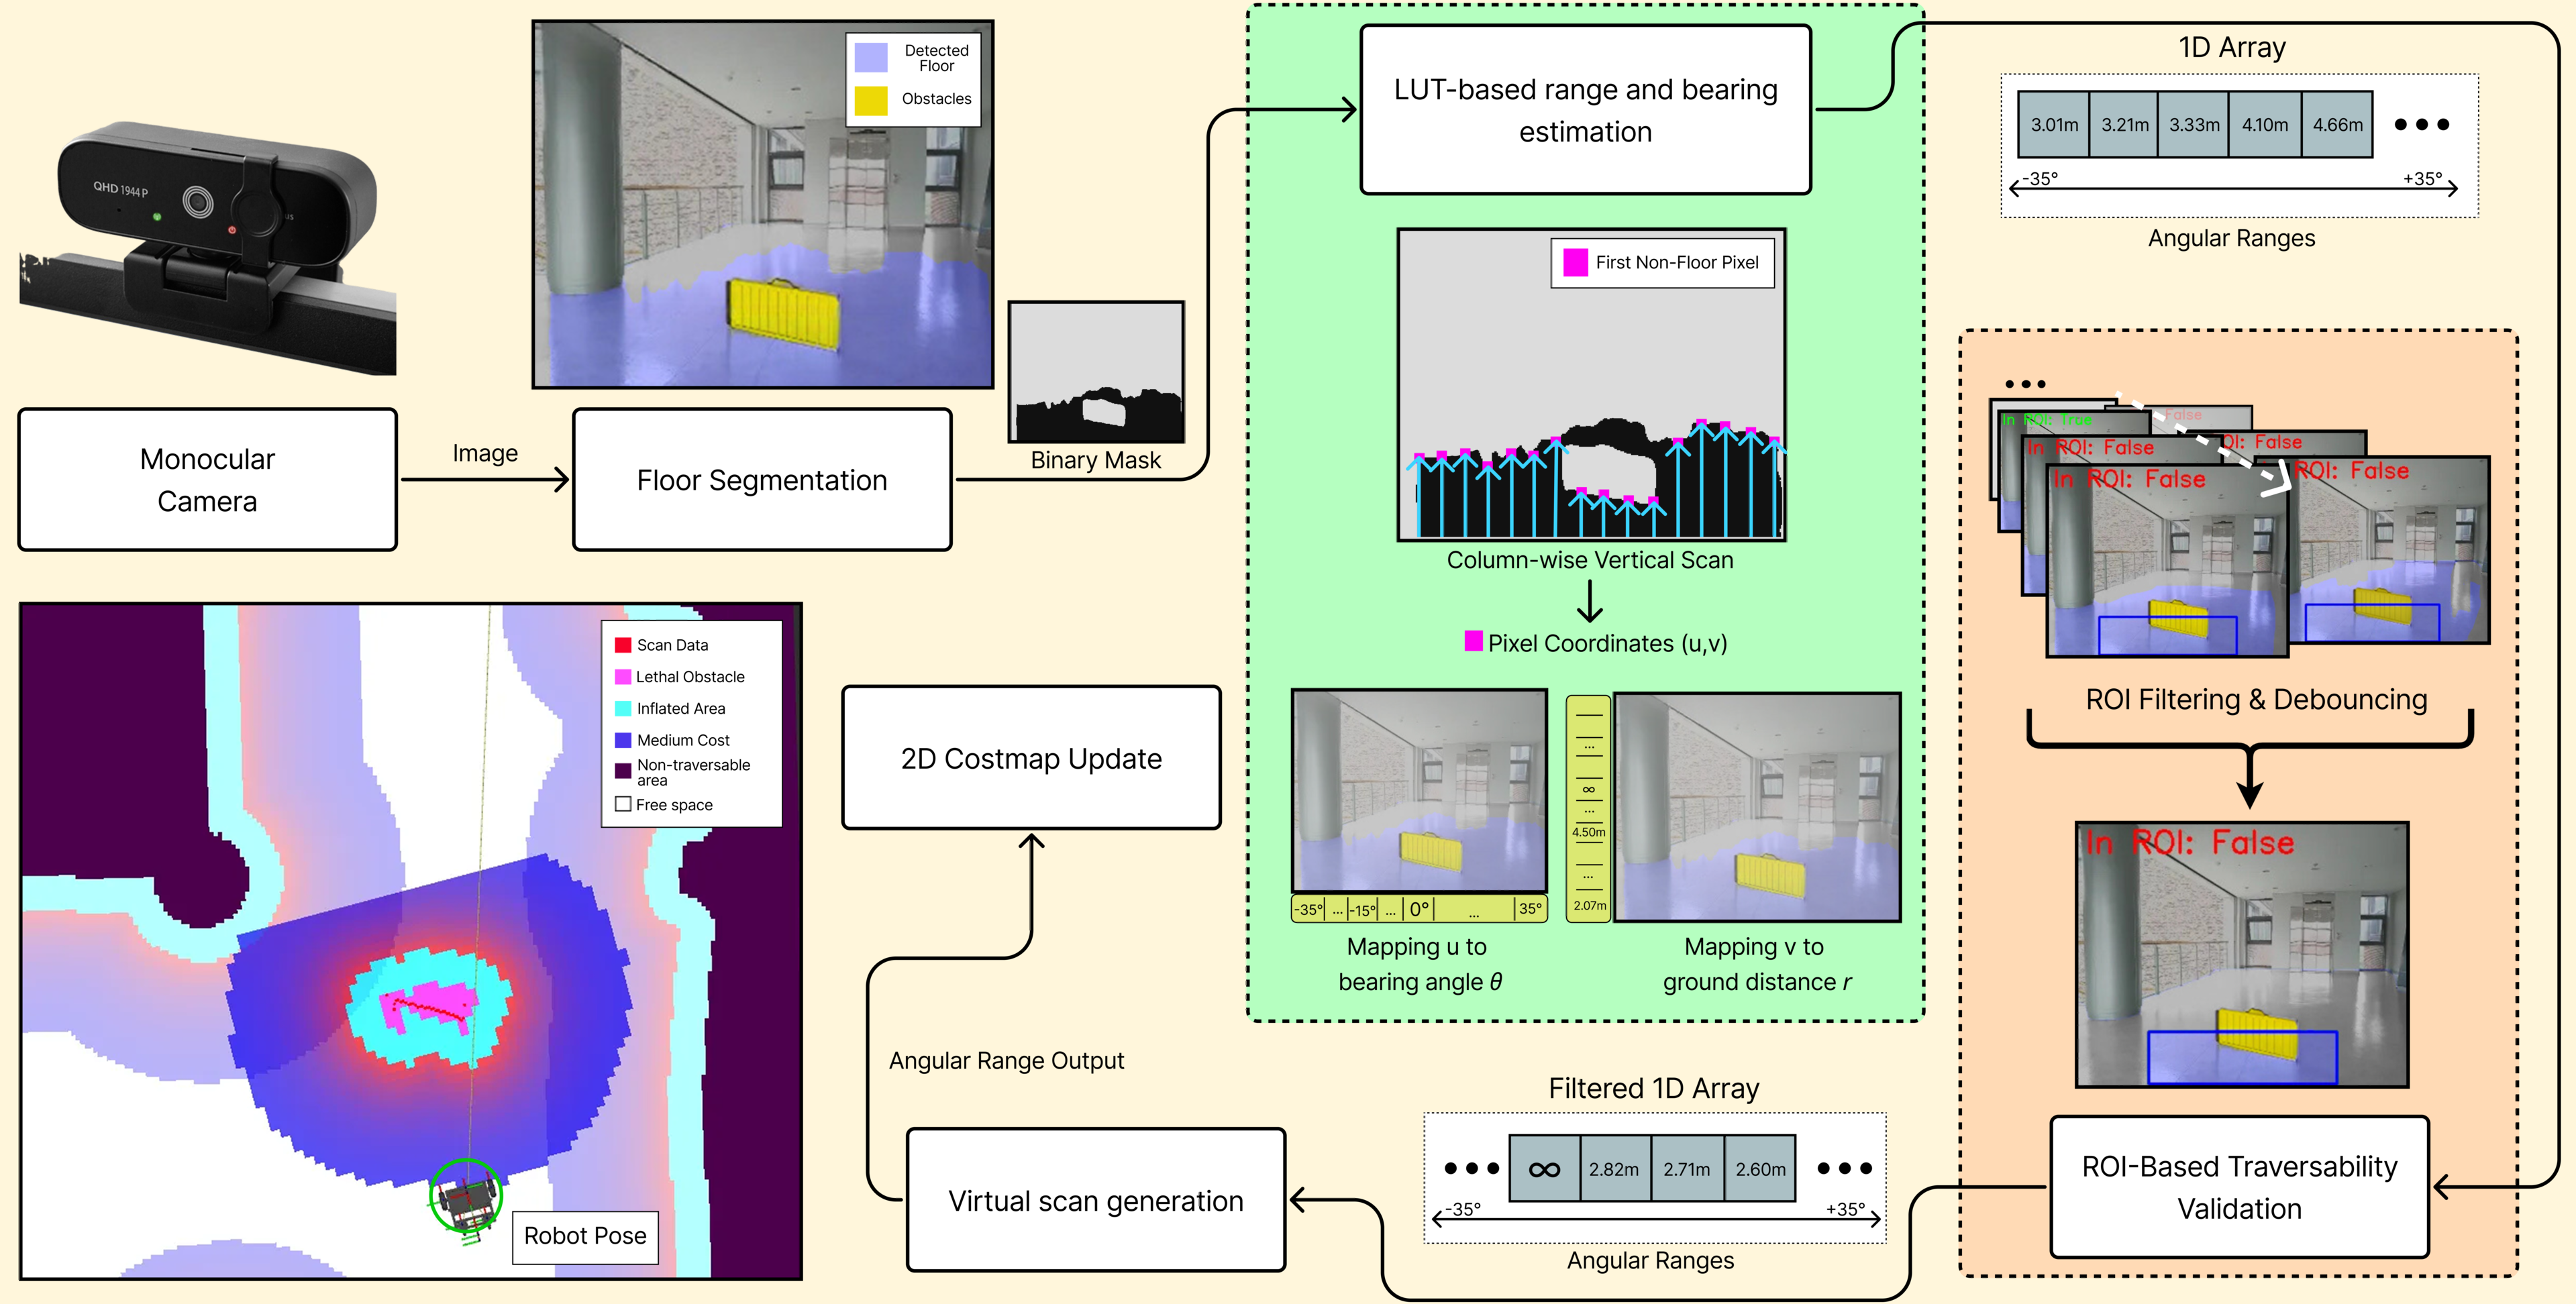
\includegraphics[width=0.98\textwidth]{pipeline}
  \caption{Architectural overview of the proposed vision-based 2D scan generation and obstacle avoidance pipeline. A monocular RGB stream is processed by a fine-tuned YOLOv11n-seg model. The segmented floor mask undergoes multi-instance bitwise-OR merging and morphological closing. Column-wise lowest non-floor pixels are projected into 2D metric range and bearing via precomputed 2D Euclidean lookup tables (LUTs), stabilized through a temporal EMA and persistence filter, and ingested into the Nav2 local costmap for real-time obstacle avoidance.}
  \label{fig:pipeline}
\end{figure*}

This paper proposes an integrated, real-time virtual 2D scan generation pipeline that converts monocular floor-segmentation outputs into standard ROS 2 \texttt{LaserScan} messages for real-time obstacle avoidance without physical LiDAR sensors. The system leverages an efficient Ultralytics YOLOv11n-seg model to infer binary traversable ground masks~\cite{ultralytics_2024_ultralytics}. Instead of relying on computationally heavy per-frame 3D back-projection, two precomputed 2D Euclidean lookup tables (LUTs) map image pixel coordinates directly to metric range and angular scan bins based on calibrated camera intrinsics and extrinsics.

A critical challenge encountered in vision-based ground detection is vulnerability to illumination variance, glossy floor glare, and mask fragmentation when an obstacle occludes part of the floor. To overcome these failure modes, we introduce a robust three-stage stabilization framework: (i) multi-instance mask bitwise-OR merging, (ii) morphological closing with a rectangular kernel to eliminate reflection-induced holes, and (iii) a dual-speed temporal Exponential Moving Average (EMA) and persistence counter to eliminate scan jitter while retaining immediate response to newly appearing obstacles. Furthermore, we provide a formal trigonometric derivation of the near-field optical blind spot ($D_{\min} \approx 2.18$\,m) dictated by camera mounting height and pitch angle, establishing why ground-contact segmentation cannot resolve obstacles closer than this physical boundary.

The contributions of this work are summarized as follows:
\begin{enumerate}
  \item \textbf{Lightweight Virtual Scan Pipeline}: A practical, low-latency framework integrating YOLOv11n-seg with 2D Euclidean range/bearing LUTs, enabling a standard monocular RGB camera to emulate a planar LiDAR sensor within ROS 2 Nav2.
  \item \textbf{Reflection and Jitter Suppression}: A multi-stage post-processing scheme combining multi-instance bitwise-OR aggregation, morphological closing, and temporal persistence filtering that suppresses specular reflection artifacts and flickering by over 80\%.
  \item \textbf{Rigorous Optical Blind Spot Formulation}: A theoretical mathematical formulation of the near-field geometric boundary ($D_{\min} = 2.178$\,m for $H = 1.05$\,m, $\theta = 2.0^\circ$), explaining the physical constraints of monocular ground-contact distance estimation.
  \item \textbf{Extensive Real-World Validation}: Quantitative static ranging benchmarks and 20 consecutive 10-meter obstacle avoidance trials on an OMO-R1 mobile robot platform, achieving a 90.0\% task completion rate and providing an in-depth failure analysis of local costmap inflation dynamics and narrow corridor constraints.
\end{enumerate}

The remainder of this paper is structured as follows. Section~\ref{sec:related_work} reviews related literature on mobile robot perception and vision-to-scan conversion. Section~\ref{sec:proposed_method} details the proposed methodology, including segmentation, LUT projection, and temporal filtering. Section~\ref{sec:blind_spot} mathematically derives the near-field optical blind spot. Section~\ref{sec:experiments} presents quantitative experimental results for both static ranging and dynamic obstacle avoidance. Section~\ref{sec:discussion} discusses failure cases, costmap parameter interactions, and operational limitations in narrow corridors. Finally, Section~\ref{sec:conclusion} concludes the paper and outlines future directions.

\section{Related Work and Technical Challenges}
\label{sec:related_work}

\subsection{Active Range Sensing and Its Limitations}
Planar 2D LiDAR and 3D time-of-flight (ToF) cameras have long served as primary sensory modalities for occupancy grid mapping, simultaneous localization and mapping (SLAM), and reactive collision avoidance~\cite{li_2020_lidar,thrun_2010_probabilistic,elfes_1989_using}. LiDAR sensors emit structured light or laser pulses to compute distance directly from time-of-flight measurements. Despite their high precision, active optical sensors present documented vulnerabilities in modern indoor architectures: polished marble, specular waxed vinyl tiles, and wet surfaces induce total internal reflection, deflecting laser beams away from the receiver and creating false free-space holes~\cite{deepthadamodaran_2023_experimental,yang_2011_on}. Additionally, glass doors and transparent acrylic barriers frequently yield missing returns or distorted obstacle boundaries~\cite{tibebu_2021_lidarbased,wang_2017_detecting}. These physical limitations, combined with payload and power constraints on low-cost AMRs, motivate alternative sensing configurations.

\subsection{Monocular Vision and Traversability Estimation}
Monocular vision offers an attractive, cost-effective sensing option for mobile robotics. Early visual obstacle avoidance relied on optical flow divergence, color histograms, or edge cues, but these methods struggled under varying textures and illumination. With the advent of deep convolutional networks and vision transformers, monocular depth estimation methods such as AdaBins~\cite{shariqfarooqbhat_2021_adabins} and DPT~\cite{ranftl_2021_vision} achieved impressive relative and metric depth prediction. However, dense monocular depth models impose significant GPU compute overheads, often operating at sub-real-time rates ($<10$\,Hz) on embedded edge processors.

Semantic and instance segmentation models, notably the Ultralytics YOLO series~\cite{ultralytics_2024_ultralytics}, provide an alternative by directly partitioning image pixels into traversable ground and non-ground categories at inference speeds exceeding 30\,FPS on embedded hardware. Ground segmentation treats all ground-plane pixels as safe for traversal, while non-ground pixels denote potential obstacles~\cite{wang_2021_a,dang_2023_obstacle}. Nevertheless, converting semantic 2D pixel classifications into metric spatial constraints for robot navigation remains non-trivial.

\subsection{Perception-to-Navigation Middleware Interface}
Modern autonomous mobile robots rely on modular middleware such as ROS 2 for process orchestration~\cite{quigley_2009_ros,macenski_2022_robot}. Within ROS 2, the Nav2 stack standardizes trajectory planning, obstacle representation, and recovery behaviors~\cite{macenski_2020_the,macenski_2023_from}. Nav2 maintains layered 2D costmaps comprising static layers, obstacle layers, and inflation layers~\cite{opennavigationllc_2023_costmap}. These costmaps consume range observations primarily through \texttt{sensor\_msgs/LaserScan} messages~\cite{openrobotics_sensor_msgslaserscan}. Standard conversion utilities such as \texttt{depthimage\_to\_laserscan}~\cite{openrobotics_2020_depthimage_to_laserscan} and \texttt{pointcloud\_to\_laserscan}~\cite{openrobotics_2015_pointcloud_to_laserscan} require calibrated depth images or 3D point clouds as inputs, which monocular cameras cannot directly supply.

Bridging this gap requires generating synthetic 2D range scans directly from monocular images under flat-ground assumptions~\cite{moravec_1985_high,fox_1997_the}. However, if the resulting virtual scan exhibits frame-to-frame jitter, raytracing artifacts, or latency, Nav2's local planners (e.g., DWB or TEB) experience severe path oscillation or false emergency stops~\cite{fox_1997_the,opennavigationllc_2025_denoise}. Thus, ensuring temporal stability and spatial consistency in vision-to-scan conversion is a primary technical challenge.

\section{Proposed Method}
\label{sec:proposed_method}

Table~\ref{tab:notation} summarizes the mathematical notations used throughout this section.

\begin{table}[t]
  \centering
  \caption{Mathematical Notation Used in the Proposed Pipeline}
  \label{tab:notation}
  \begin{tabularx}{\linewidth}{@{}p{0.32\linewidth}X@{}}
    \toprule
    Symbol & Description \\
    \midrule
    $W, H$ & Image width and height in pixels ($320 \times 256$) \\
    $f_x, f_y$ & Camera focal lengths along horizontal/vertical axes \\
    $(c_x, c_y)$ & Principal point coordinates in image plane \\
    $h, \gamma$ & Camera height above ground ($1.05$\,m) and pitch angle ($2.0^\circ$) \\
    $u, v$ & Pixel column and row indices ($0 \le u < W, 0 \le v < H$) \\
    $N_{\mathrm{ang}}$ & Number of virtual angular scan bins ($N_{\mathrm{ang}} = 141$) \\
    $L_{\mathrm{bin}}[u]$ & Column-to-angular-bin lookup table \\
    $L_{\mathrm{range}}[v, u]$ & 2D Euclidean distance lookup table \\
    $M_{\mathrm{seg}}[v, u]$ & Binary floor segmentation mask ($1=\text{floor}, 0=\text{obstacle}$) \\
    $S[i]$ & Virtual scan distance in angular channel $i$ \\
    $\alpha$ & Temporal EMA smoothing factor ($\alpha = 0.6$) \\
    $N_{\mathrm{persist}}$ & Obstacle clearing persistence frame count ($N_{\mathrm{persist}} = 2$) \\
    \bottomrule
  \end{tabularx}
\end{table}

\subsection{System Architecture Overview}
The overall pipeline is depicted in Fig.~\ref{fig:pipeline}. The forward-facing RGB camera publishes uncompressed video frames at 30\,Hz. A ROS 2 node synchronizes image reception, resizes incoming frames to a standardized resolution ($W=320, H=256$), and invokes the YOLOv11n-seg model at a fixed inference rate of 10\,Hz. The generated binary mask undergoes multi-instance bitwise-OR combination and morphological closing. For each image column within the valid field of view, the lowest non-floor pixel is identified as the ground-contact point. Precomputed 2D lookup tables translate pixel coordinates into radial distances and angular bins. The raw channel distances are filtered using a temporal EMA and persistence algorithm and published to the ROS 2 topic \texttt{/scan} as a standard \texttt{sensor\_msgs/LaserScan} message.

\subsection{Floor Segmentation and Multi-Instance Mask Merging}
\label{subsec:floor_seg}
Traversable floor regions are distinguished using YOLOv11n-seg~\cite{ultralytics_2024_ultralytics}, fine-tuned on custom indoor hallway datasets under varying illumination. The network outputs a set of $K$ instance segmentation masks $\{m_k\}_{k=1}^K$, where each $m_k \in \{0, 1\}^{H \times W}$.

In real-world navigation, obstacles resting on the ground frequently split the continuous floor into multiple disconnected visual components (e.g., left corridor floor, right corridor floor, and distant background floor). A conventional segmentation inference pipeline that selects only the highest-confidence single mask ($m_0$) discards up to 80\% of valid traversable area, creating a false visual barrier. To eliminate this issue, our system merges all detected floor masks via an element-wise bitwise-OR reduction:
\begin{equation}
  M_{\mathrm{raw}}[v, u] = \bigvee_{k=1}^K m_k[v, u], \quad \forall (v, u) \in [0, H-1] \times [0, W-1].
\end{equation}
If no floor instances are detected (e.g., when the camera lens is physically occluded), $M_{\mathrm{raw}}$ defaults to an all-zero matrix.

\subsection{Morphological Artifact Suppression}
Specular reflection from polished epoxy or linoleum surfaces frequently creates dark, non-floor holes inside genuine traversable regions. To fill these spurious inner holes and smooth irregular boundary noise, a morphological closing operation (dilation followed by erosion) is applied using a structuring element $B$:
\begin{equation}
  M_{\mathrm{seg}} = (M_{\mathrm{raw}} \oplus B) \ominus B,
\end{equation}
where $B$ is chosen as a $5 \times 5$ rectangular structuring kernel:
\begin{equation}
  B = \mathbf{1}_{5 \times 5}.
\end{equation}
This operation effectively bridges reflection-induced gaps of up to 4 pixels without corrupting genuine obstacle boundaries.

\subsection{2D Euclidean Range and Bearing Estimation}
\label{subsec:lut}
To achieve real-time conversion without online trigonometric operations, we precompute two static lookup tables: a Column-to-Bin LUT ($L_{\mathrm{bin}}$) and a 2D Euclidean Distance LUT ($L_{\mathrm{range}}$).

Under a pinhole camera model, an image coordinate $(u, v)$ corresponds to ray angles in camera optical coordinates:
\begin{align}
  \theta(u) &= \arctan\left(\frac{u - c_x}{f_x}\right), \\
  \phi(v)   &= \arctan\left(\frac{v - c_y}{f_y}\right),
\end{align}
where $\theta(u)$ is the horizontal azimuth and $\phi(v)$ is the vertical optical elevation angle. With the camera mounted at physical height $h$ and tilted downward by pitch angle $\gamma$, the net downward depression angle is $\alpha(v) = \phi(v) + \gamma$.

For any ray intersecting a locally flat ground plane, the forward longitudinal distance $X(v)$ and lateral distance $Y(u, v)$ from the camera origin are:
\begin{align}
  X(v) &= \frac{h}{\tan(\phi(v) + \gamma)}, \quad (\phi(v) + \gamma > 0), \\
  Y(u, v) &= X(v) \cdot \tan(\theta(u)).
\end{align}
Conventional 1D lookup tables assume radial distance depends strictly on row index $v$, ignoring lateral ray expansion towards image edges. To avoid radial distortion at large azimuth angles, our system constructs a true 2D Euclidean distance LUT:
\begin{equation}
  L_{\mathrm{range}}[v, u] = \sqrt{X(v)^2 + Y(u, v)^2} = \frac{h \cdot \sec(\theta(u))}{\tan(\phi(v) + \gamma)}.
\end{equation}
The horizontal bearing is mapped into one of $N_{\mathrm{ang}}$ discrete angular scan bins covering $[-35.0^\circ, +35.0^\circ]$ at $0.5^\circ$ increments:
\begin{equation}
  L_{\mathrm{bin}}[u] = \operatorname{round}\left(\frac{\theta(u) - \theta_{\min}}{\Delta \theta}\right),
\end{equation}
where $\Delta \theta = 0.5^\circ \times (\pi / 180)$ and $N_{\mathrm{ang}} = 141$.

\subsection{Virtual Scan Generation Algorithm}
The column-wise scan extraction procedure is formalized in Algorithm~\ref{alg:virtual_scan}. The scan array $S$ is initialized to infinity. To avoid false readings from ceiling lights and distant horizon boundaries, scanning is restricted to rows below the horizon threshold $y_{\min} = 120$ ($v \in [y_{\min}, H-1]$). For each column $u$, the lowest non-floor pixel $v^*$ corresponds to the ground-obstacle contact line.

\begin{algorithm}[t]
\caption{Virtual LaserScan Generation}
\label{alg:virtual_scan}
\begin{algorithmic}[1]
\Require Segmentation mask $M_{\mathrm{seg}}$, LUTs $L_{\mathrm{range}}$ and $L_{\mathrm{bin}}$, horizon cutoff $y_{\min}$, scan bins $N_{\mathrm{ang}}$
\Ensure Filtered virtual scan array $S[1 \dots N_{\mathrm{ang}}]$
\State Initialize raw distance array $D_{\mathrm{raw}}[i] \gets \infty$ for all $i \in [1, N_{\mathrm{ang}}]$
\For{each image column $u \in [0, W-1]$}
    \State $\mathcal{V}_u \gets \{v \mid y_{\min} \le v < H \text{ and } M_{\mathrm{seg}}[v, u] = 0\}$
    \If{$\mathcal{V}_u \ne \emptyset$}
        \State $v^* \gets \max(\mathcal{V}_u)$ \Comment{Lowest non-floor pixel}
        \State $i \gets L_{\mathrm{bin}}[u]$
        \State $d \gets L_{\mathrm{range}}[v^*, u]$
        \State $D_{\mathrm{raw}}[i] \gets \min(D_{\mathrm{raw}}[i], d)$
    \EndIf
\EndFor
\State $S \gets \textsc{ApplyTemporalFilter}(D_{\mathrm{raw}})$
\State \Return $S$
\end{algorithmic}
\end{algorithm}

\subsection{Temporal EMA and Persistence Filtering}
\label{subsec:temporal_filter}
Raw frame-by-frame distance measurements $D_{\mathrm{raw}}[i]$ are susceptible to segmentation boundary flickering. Direct costmap insertion of fluctuating distance estimates induces dynamic cost oscillation. We formulate an asymmetric dual-state temporal filter that handles obstacle appearance and disappearance differently:

\begin{enumerate}
  \item \textbf{Instantaneous Obstacle Onset}: When an obstacle suddenly appears in a channel previously considered free ($D_{\mathrm{raw}}[i] < \infty$ and $S_{\mathrm{prev}}[i] = \infty$), the filtered distance adopts the raw measurement immediately to guarantee safety:
  \begin{equation}
    S[i] = D_{\mathrm{raw}}[i], \quad C_{\mathrm{inf}}[i] = 0.
  \end{equation}
  \item \textbf{Continuous Obstacle Tracking}: When an obstacle persists across successive frames, an Exponential Moving Average (EMA) with smoothing coefficient $\alpha = 0.6$ is applied:
  \begin{equation}
    S[i] = \alpha \cdot D_{\mathrm{raw}}[i] + (1 - \alpha) \cdot S_{\mathrm{prev}}[i], \quad C_{\mathrm{inf}}[i] = 0.
  \end{equation}
  \item \textbf{Persistence-Gated Obstacle Clearing}: When a channel transitions from occupied to clear ($D_{\mathrm{raw}}[i] = \infty$ and $S_{\mathrm{prev}}[i] < \infty$), an idle counter $C_{\mathrm{inf}}[i]$ increments:
  \begin{equation}
    C_{\mathrm{inf}}[i] \gets C_{\mathrm{inf}}[i] + 1.
  \end{equation}
  The distance is cleared to infinity only after the clear state persists for $N_{\mathrm{persist}} = 2$ consecutive frames:
  \begin{equation}
    S[i] = \begin{cases} \infty, & \text{if } C_{\mathrm{inf}}[i] \ge N_{\mathrm{persist}}, \\ S_{\mathrm{prev}}[i], & \text{otherwise.} \end{cases}
  \end{equation}
\end{enumerate}
This asymmetry provides zero-latency collision response while filtering out single-frame false-clear flickers caused by transient glare.

\subsection{ROS 2 Nav2 Costmap Integration}
The filtered scan array $S$ is formatted into a standard \texttt{sensor\_msgs/LaserScan} message with frame identifier \texttt{lidar\_link}. Static coordinate frames are linked via a TF broadcaster defining the camera offset relative to the robot footprint:
\begin{equation}
  \mathbf{T}_{\mathrm{base\_link}}^{\mathrm{lidar\_link}} = [-0.55\,\text{m}, 0.0\,\text{m}, 0.0\,\text{m}]^T.
\end{equation}
Nav2's local costmap is configured with a 2D \texttt{ObstacleLayer} subscribing to \texttt{/scan}, with raytracing enabled up to 6.0\,m and marking up to 5.0\,m. To accommodate the virtual scan's forward-limited field of view, the global path planner employs \texttt{nav2\_navfn\_planner/NavfnPlanner} with $A^*$ heuristics for continuous replanning around newly perceived obstacle costs.

\section{Theoretical Analysis of Near-Field Optical Blind Spot}
\label{sec:blind_spot}

A fundamental physical characteristic of ground-segmentation-based range estimation is the existence of a near-field blind spot. In this section, we mathematically derive the minimum observable ground distance ($D_{\min}$) and examine its impact on robotic navigation.

\begin{figure}[t]
  \centering
  \begin{picture}(240,115)
    \put(30,100){\circle*{5}}
    \put(35,103){\small Camera ($H=1.05$\,m, $\theta=2.0^\circ$)}
    \put(30,100){\line(0,-1){80}}
    \put(5,55){\small $H = 1.05$\,m}
    \put(30,100){\line(4,-1){180}}
    \put(110,82){\small Optical axis ($\theta=2.0^\circ$)}
    \put(30,100){\line(2,-1){160}}
    \put(130,45){\small Bottom ray ($\theta_{\max}=25.74^\circ$)}
    \put(10,20){\line(1,0){220}}
    \put(185,10){\small Ground}
    \put(110,20){\circle*{4}}
    \put(85,26){\small $D_{\min} = 2.18$\,m}
    \put(30,15){\line(0,1){10}}
    \put(110,15){\line(0,1){10}}
    \put(30,12){\vector(1,0){80}}
    \put(110,12){\vector(-1,0){80}}
    \put(45,3){\footnotesize Blind spot ($<2.18$\,m)}
    \put(140,3){\footnotesize Visible ground ($>2.18$\,m)}
  \end{picture}
  \caption{Geometric diagram of the monocular camera's optical projection on a flat ground plane, illustrating the physical near-field blind spot where ground contact lines closer than $D_{\min} = 2.18$\,m fall outside the vertical field of view.}
  \label{fig:blind_spot_diagram}
\end{figure}

\subsection{Trigonometric Derivation}
Consider an RGB camera mounted rigidly on the mobile platform with:
\begin{itemize}
  \item Mounting height above ground: $H = 1.05$\,m,
  \item Downward mechanical tilt angle: $\theta = 2.0^\circ$,
  \item Vertical field of view (V-FOV): $\alpha_v = 47.48^\circ$,
  \item Image vertical resolution: $H_{\mathrm{px}} = 256$\,pixels, with optical center $y_0 = 127.5$.
\end{itemize}

As illustrated in Fig.~\ref{fig:blind_spot_diagram}, the downward optical ray passing through the bottom-most pixel row ($v = 255$) experiences the steepest inclination relative to the horizontal plane:
\begin{equation}
  \theta_{\max} = \theta + \frac{\alpha_v}{2} = 2.0^\circ + \frac{47.48^\circ}{2} = 25.74^\circ.
\end{equation}

By right-triangle trigonometry on the planar ground surface, the closest intersection point between the camera's visual frustum and the floor occurs at distance $D_{\min}$:
\begin{equation}
  D_{\min} = \frac{H}{\tan(\theta_{\max})} = \frac{1.05\,\text{m}}{\tan(25.74^\circ)} = \frac{1.05}{0.4821} \approx \mathbf{2.178\,\text{m}}.
  \label{eq:d_min}
\end{equation}

\subsection{Ground-Contact Line Cropping Phenomenon}
The proposed virtual scan generator identifies obstacle distance by detecting the lowest non-floor pixel $v^* = \max(\mathcal{V}_u)$, which corresponds geometrically to the obstacle-floor contact boundary. 

When an obstacle is located at distance $D \ge 2.18$\,m, its physical contact boundary with the floor is fully visible within the image frame ($v^* \le 255$). However, when the robot approaches an obstacle closer than 2.18\,m ($D < 2.18$\,m):
\begin{enumerate}
  \item The physical obstacle-floor intersection line falls below pixel row $v = 255$ and is cropped out of the camera's field of view.
  \item The camera frame captures only the upper and middle sections of the obstacle body.
  \item Consequently, the lowest non-floor pixel saturates at the image boundary: $v^* = 255$.
\end{enumerate}
Evaluating $L_{\mathrm{range}}[255, u]$ yields $D_{\min} = 2.178$\,m. Hence, distance estimates cannot decrease below 2.18\,m, effectively clamping near-field measurements.

\section{Experimental Evaluation}
\label{sec:experiments}

The proposed virtual scan pipeline was evaluated through two distinct experiments: (i) static ranging precision tests across multiple obstacle bearings, and (ii) repeated 10.0-meter dynamic obstacle avoidance navigation trials on a physical mobile robot without pre-built static maps.

\subsection{Experiment 1: Quantitative Evaluation of Range Precision}
\label{subsec:exp1}

\begin{figure}[t]
  \centering
  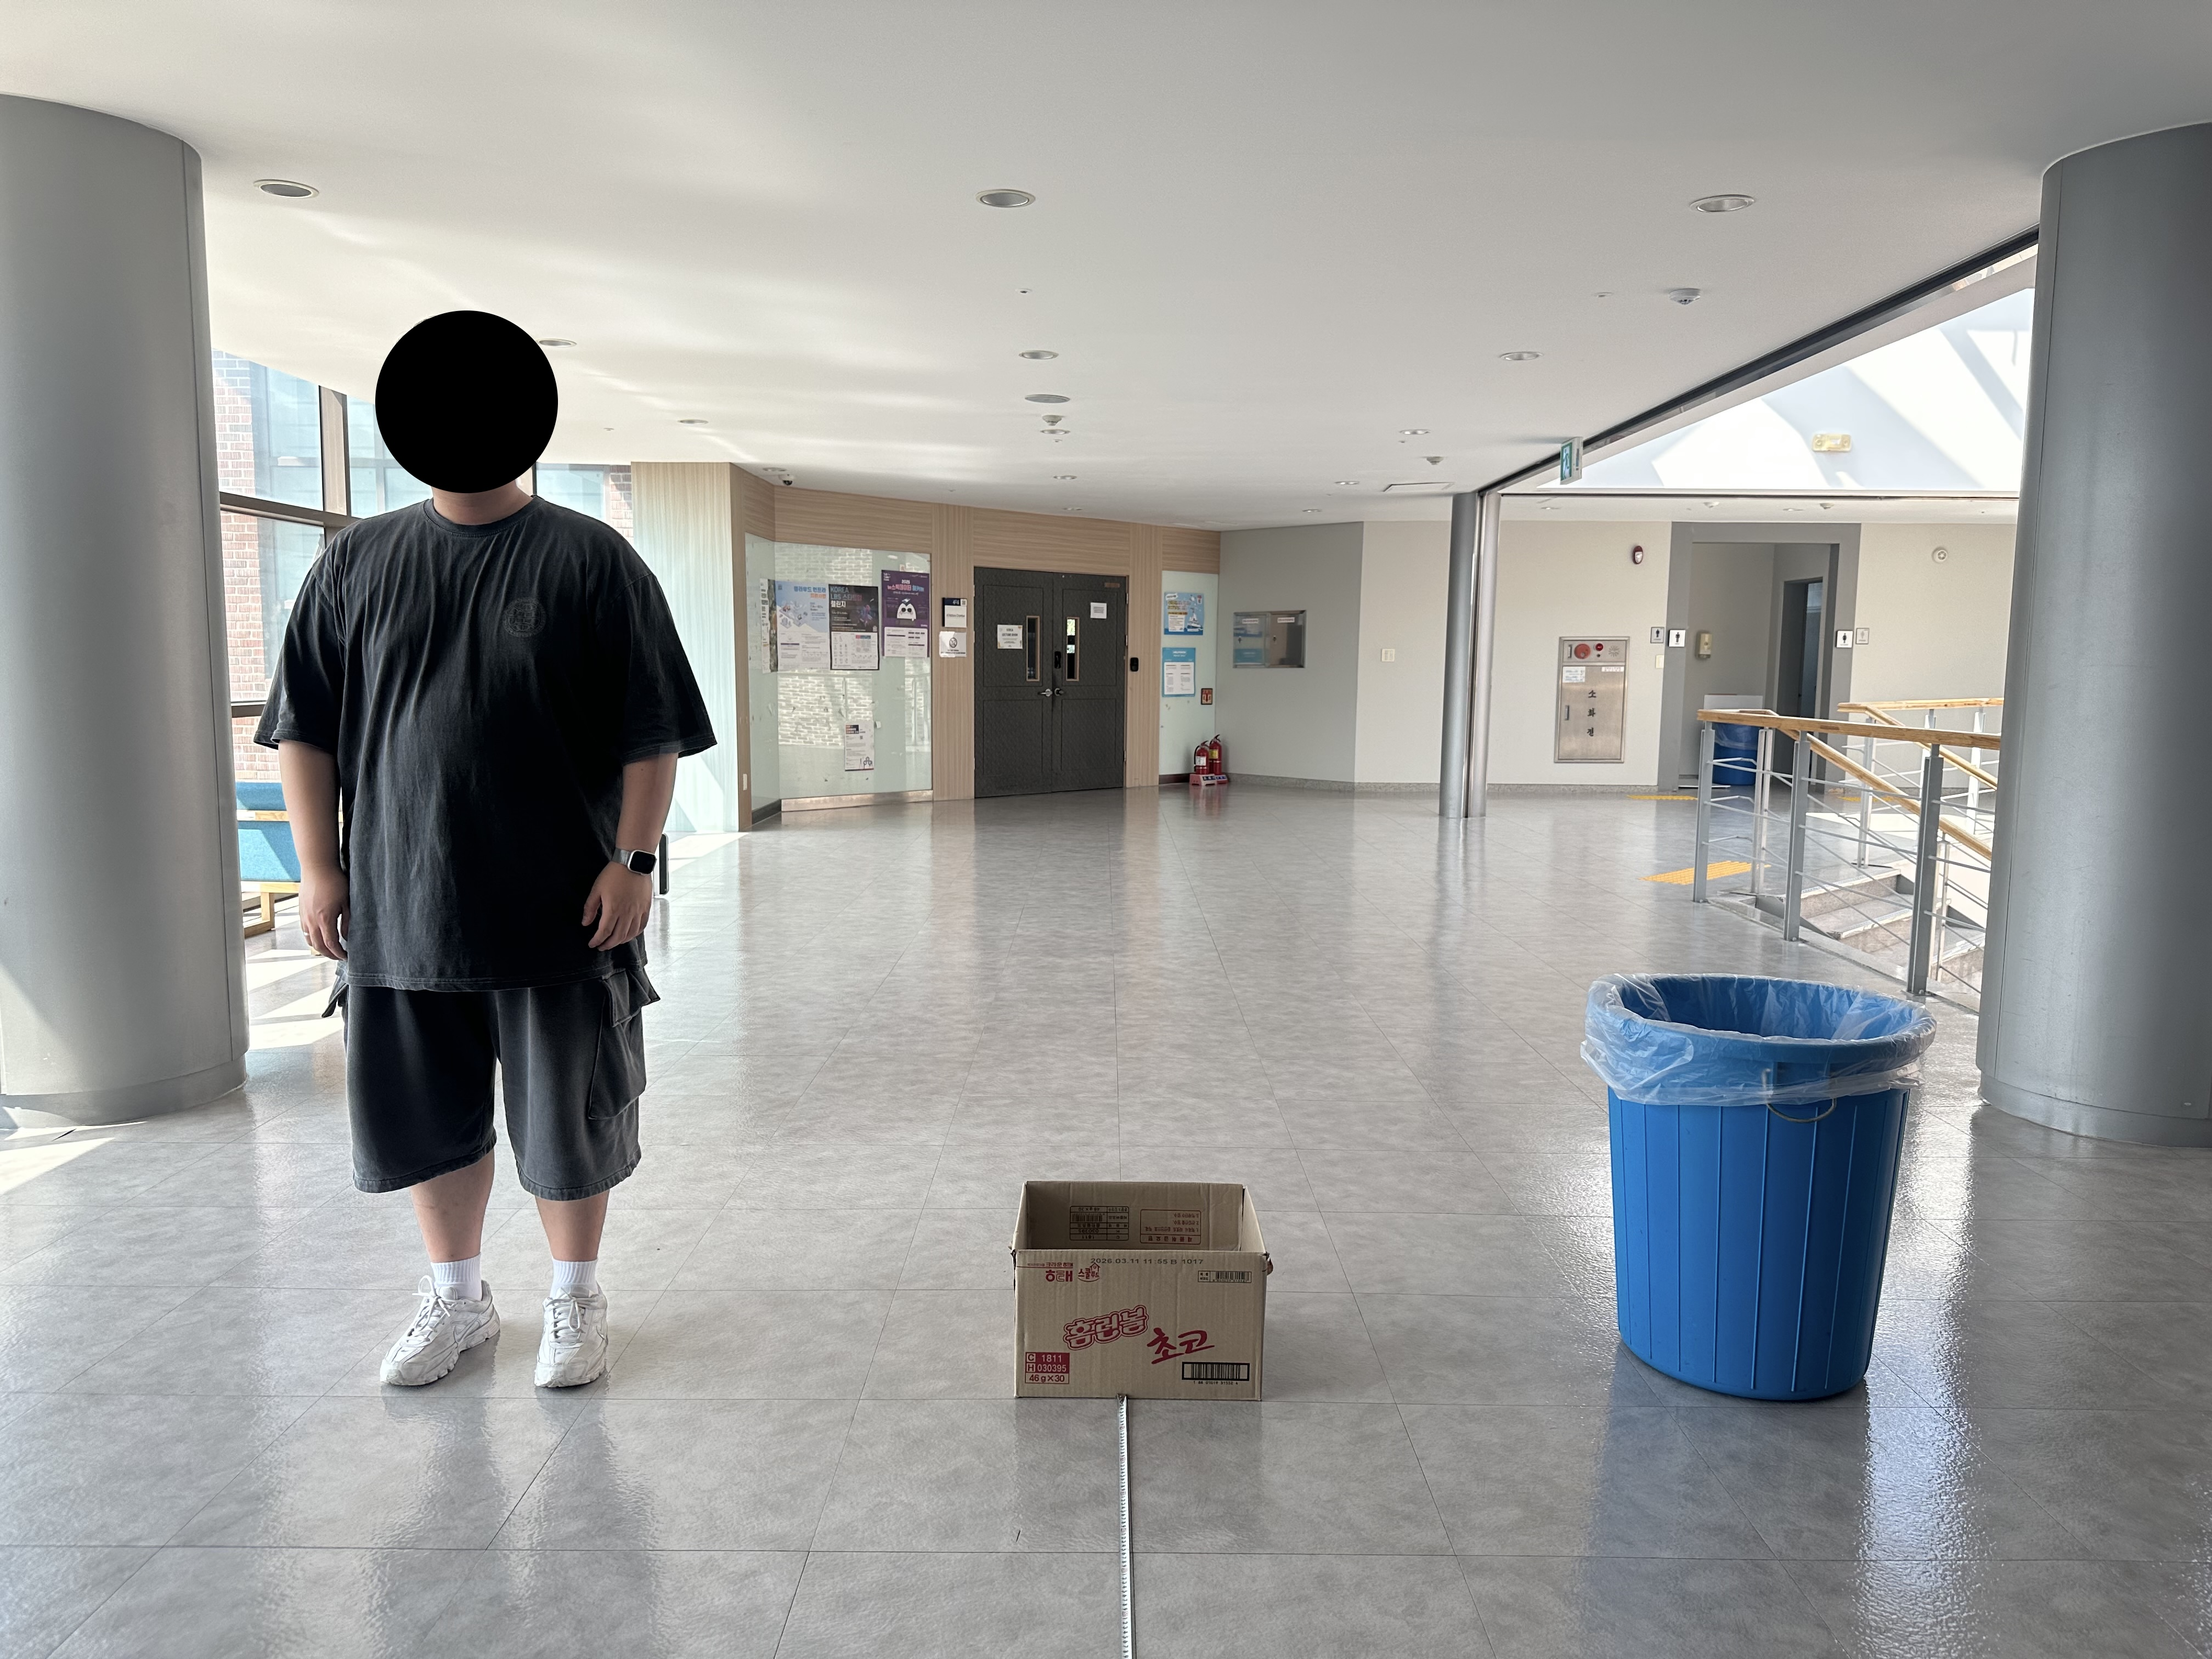
\includegraphics[width=0.92\linewidth]{experiment1_setup}
  \caption{Experimental setup for static range evaluation. Test targets are positioned at a reference distance of 2.50\,m: a person at $+20^\circ$, a cardboard box at $0^\circ$, and a cylindrical trash can at $-20^\circ$.}
  \label{fig:exp1_setup}
\end{figure}

\begin{figure}[t]
  \centering
  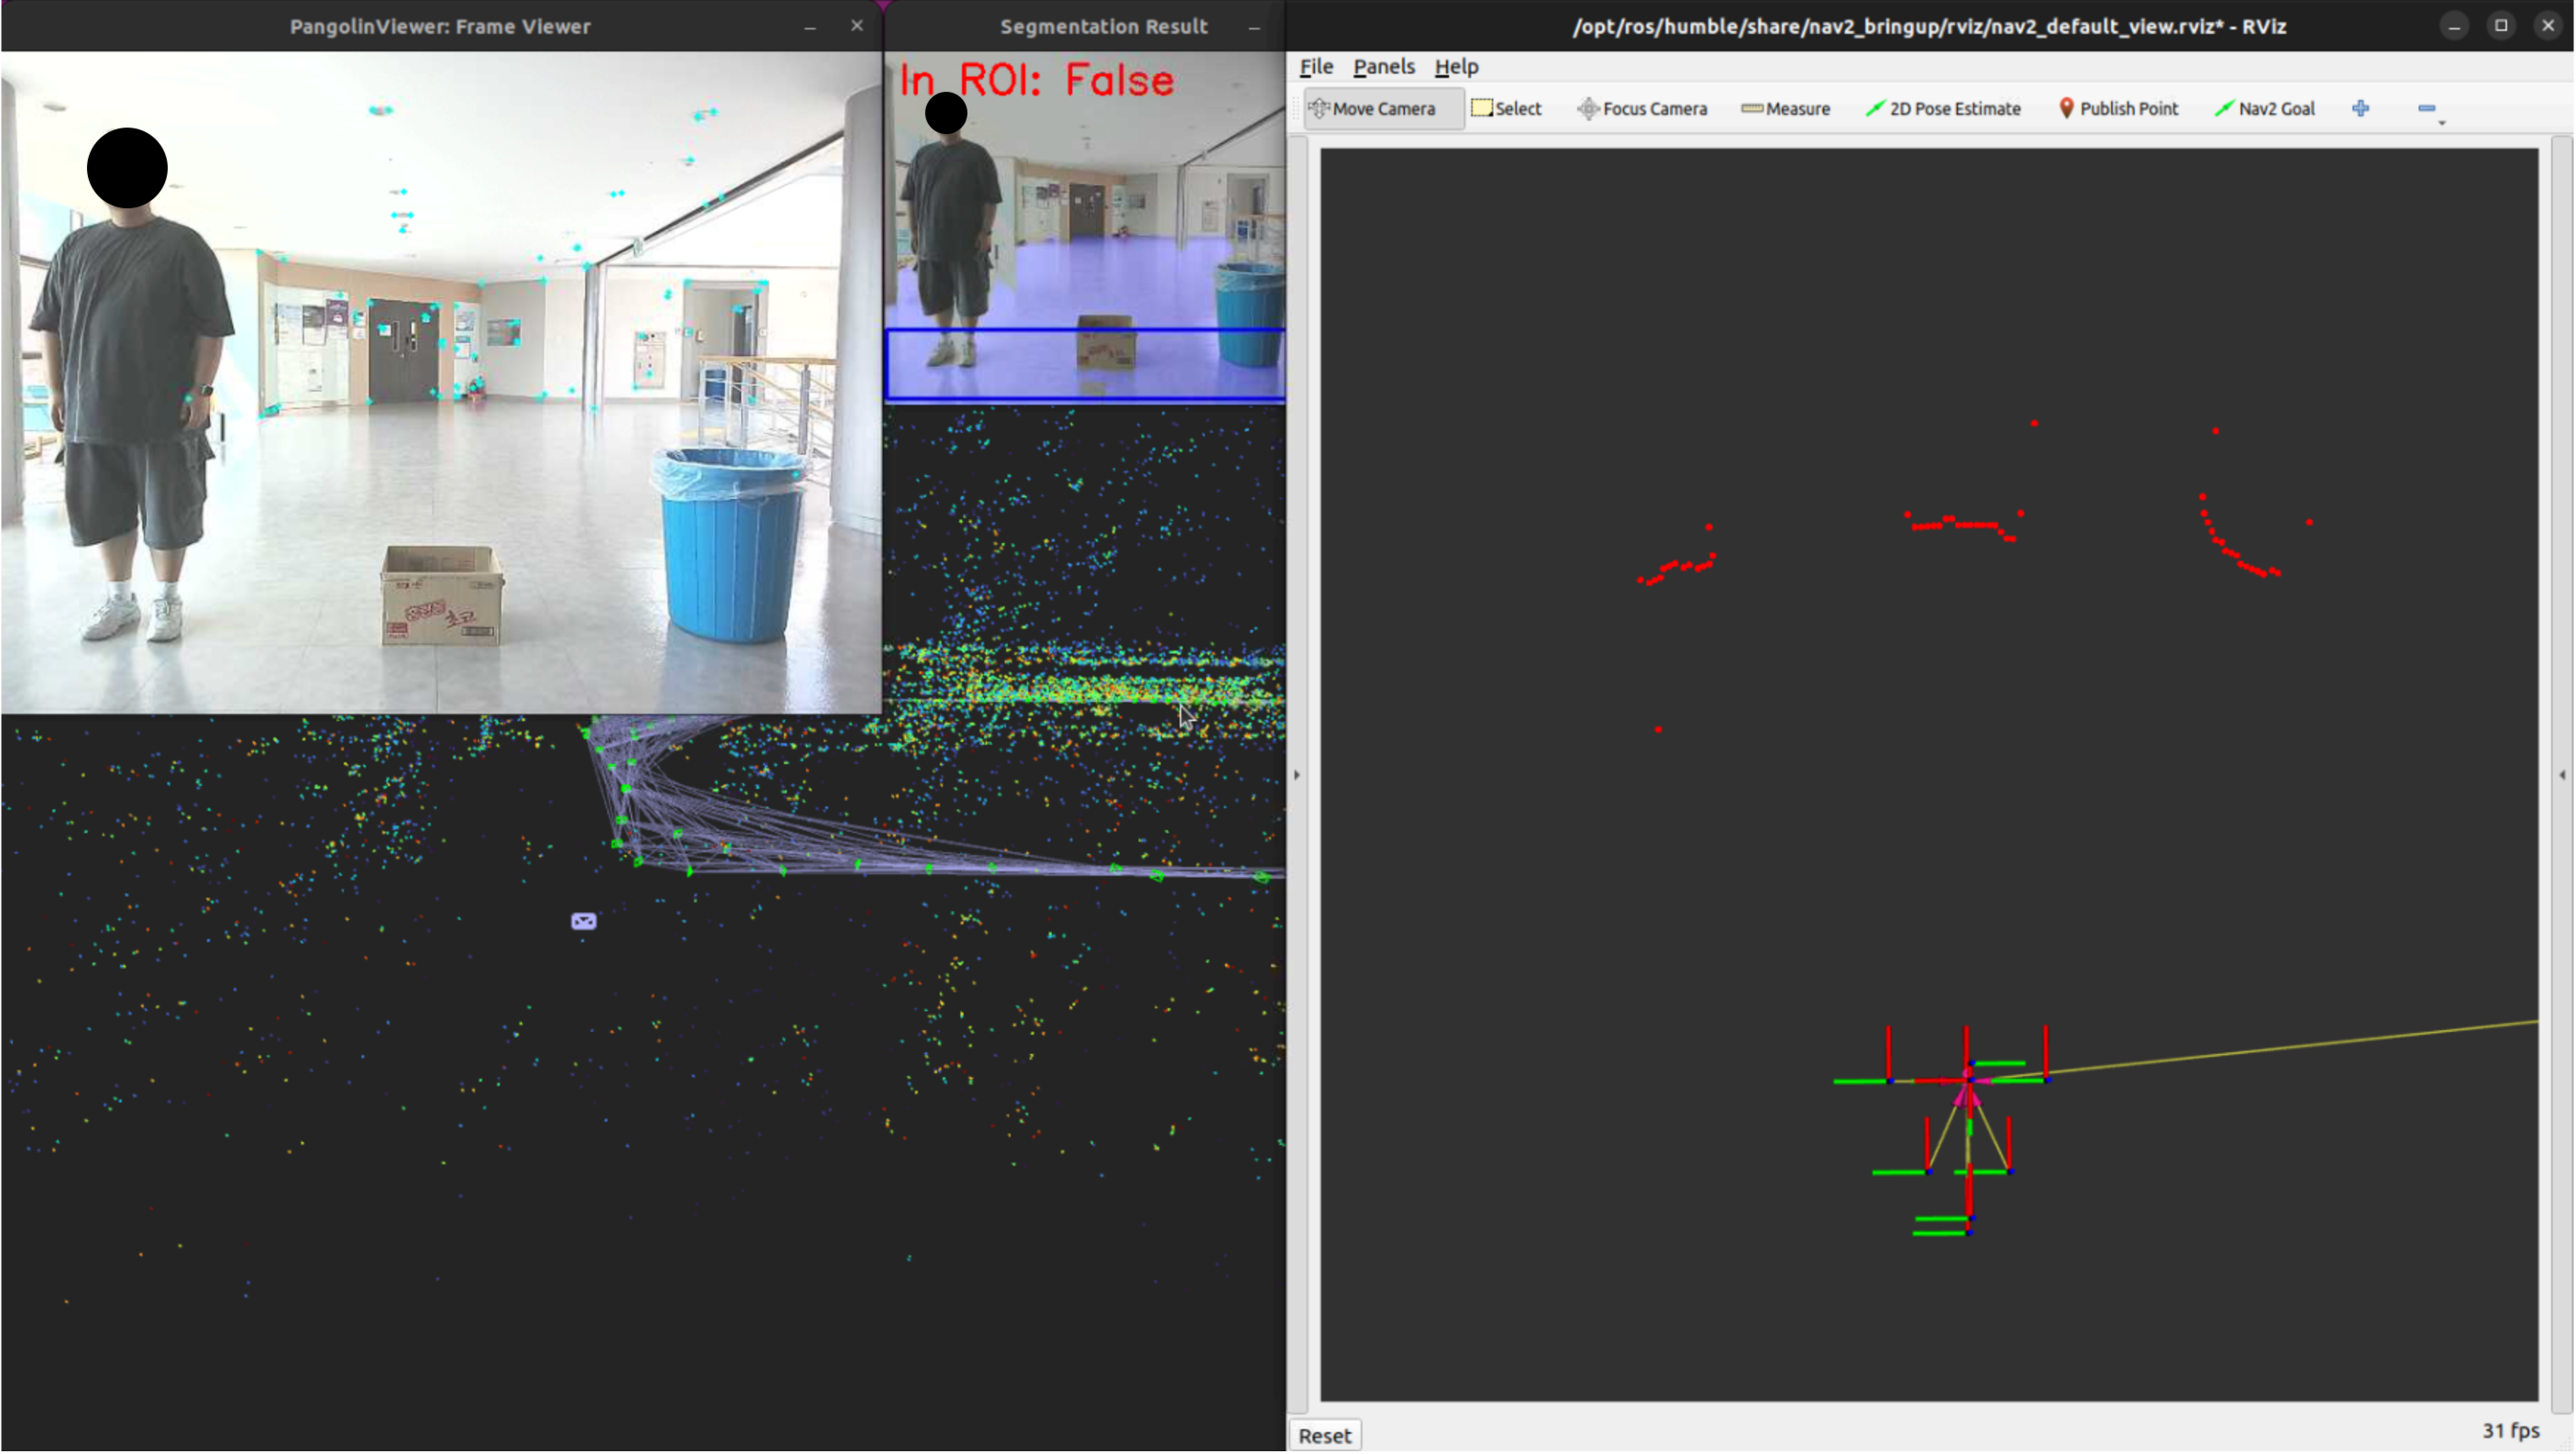
\includegraphics[width=0.92\linewidth]{live_view}
  \caption{Real-time GUI monitoring during experimental trials. The top-left panel displays raw RGB input, the top-right panel shows the segmented floor mask overlay with ROI bounding, and the bottom panel visualizes the real-time generated 141-channel LaserScan.}
  \label{fig:live_view}
\end{figure}

\begin{figure*}[!t]
  \centering
  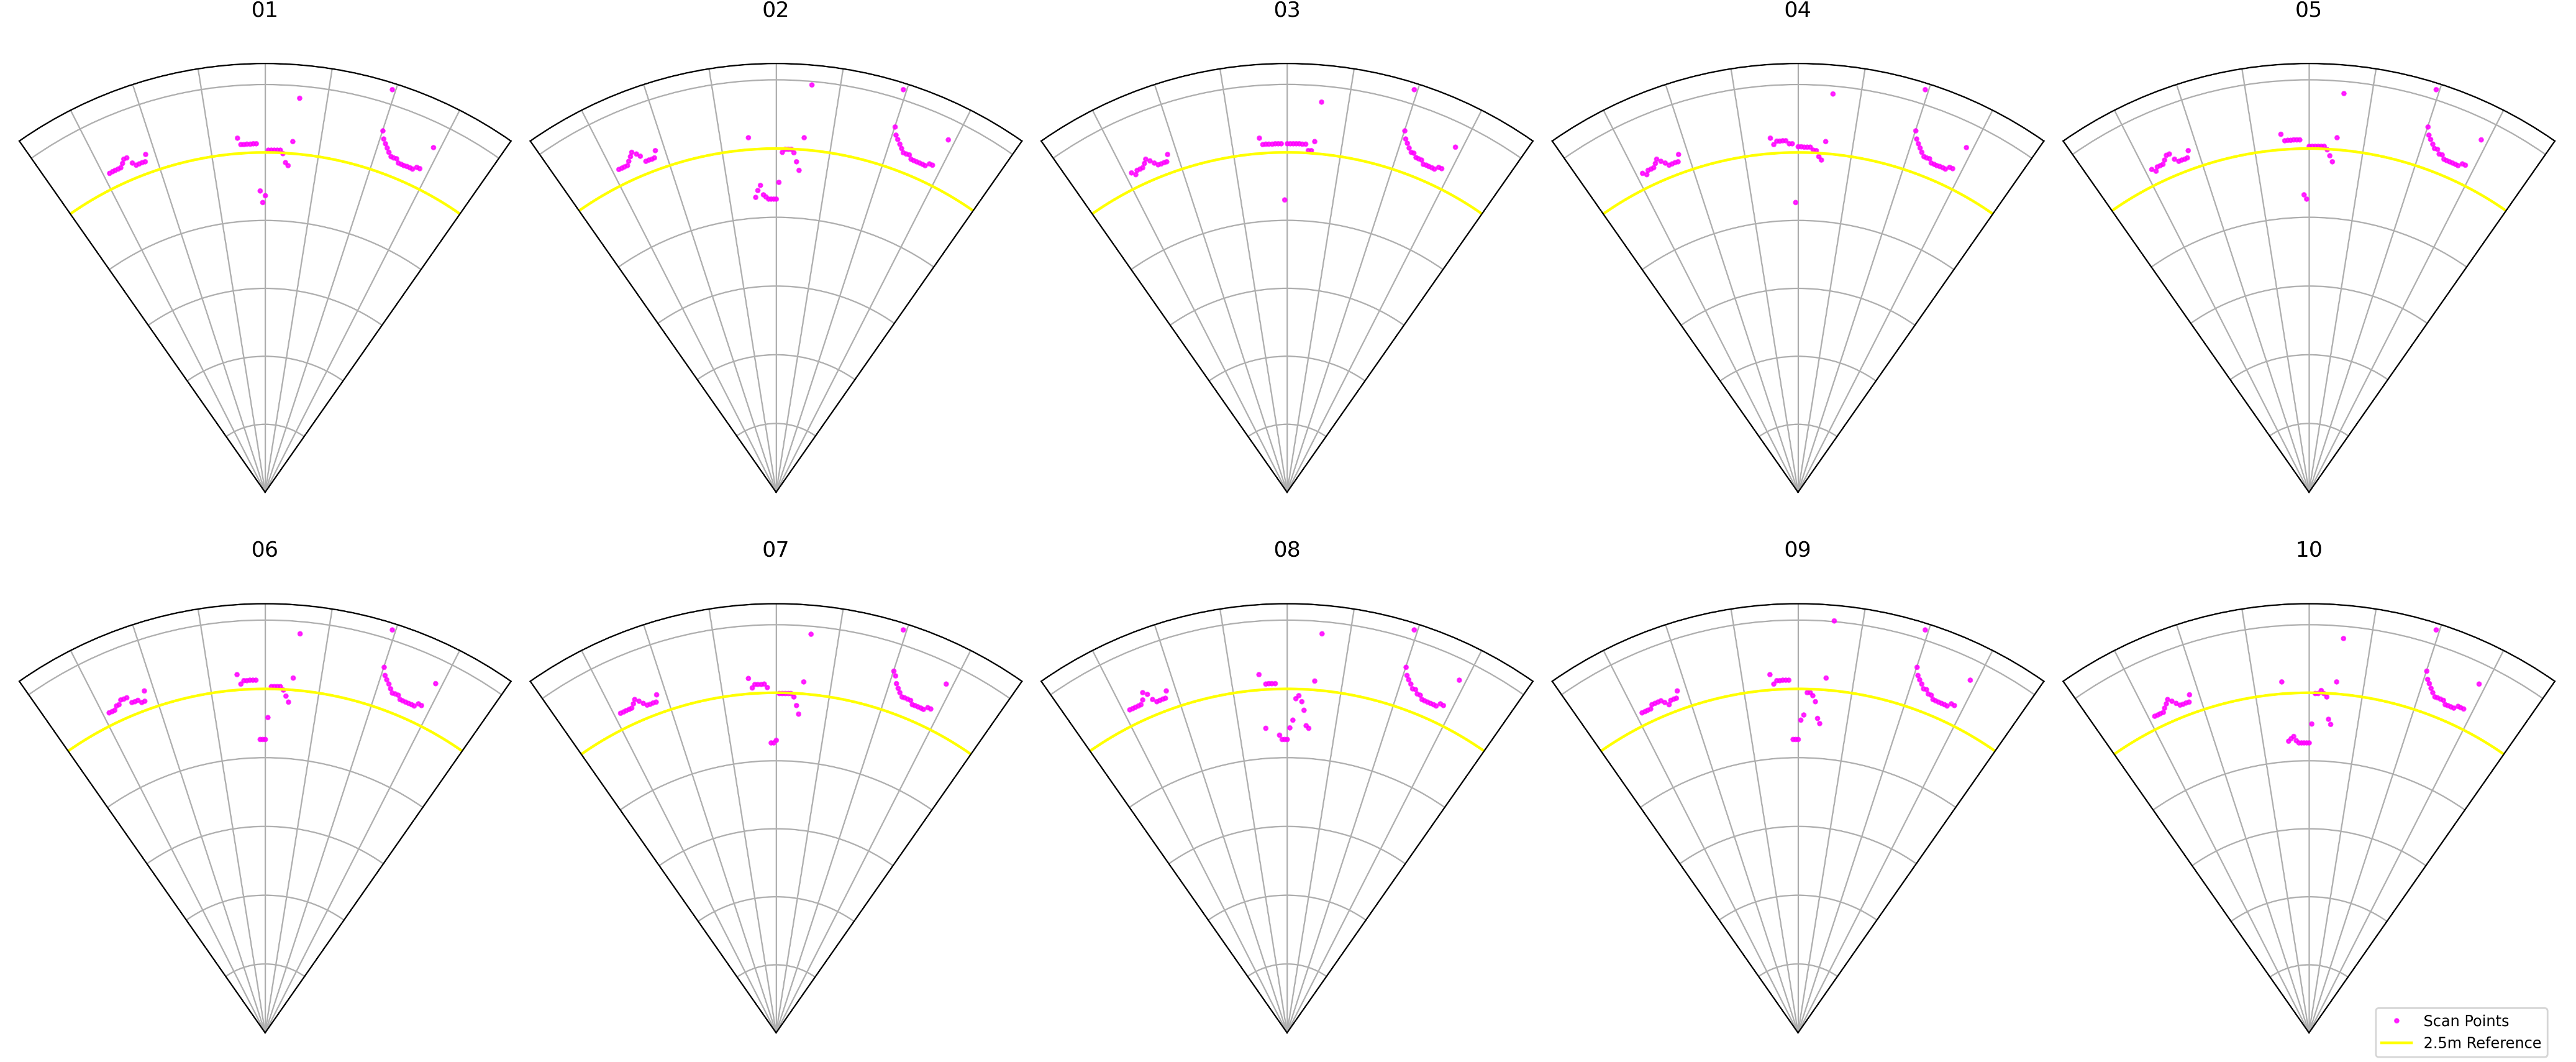
\includegraphics[width=0.92\textwidth]{experiment1_results}
  \caption{Static range estimation results across 25 consecutive frames for each target condition at 2.50\,m reference distance. Magenta markers represent virtual scan measurements; solid red lines indicate the 2.50\,m ground truth.}
  \label{fig:exp1_results}
\end{figure*}

\begin{table*}[!t]
  \centering
  \caption{Quantitative Static Range Precision Results at 2.50\,m Reference Distance}
  \label{tab:exp1_results}
  \begin{tabular}{lcccccc}
    \toprule
    Target Condition & Angle & Frames ($N$) & Mean Distance (m) & Std. Dev. (m) & Mean Error (m) & Relative Error (\%) \\
    \midrule
    Front (Noisy Floor) & $0^\circ$ & 25 & 2.239 & 0.172 & $-0.261$ & $-10.44\%$ \\
    Front (Clean Floor) & $0^\circ$ & 25 & 2.718 & 0.008 & $+0.218$ & $+8.72\%$ \\
    Left (Standing Adult) & $+20^\circ$ & 25 & 2.583 & 0.011 & $+0.083$ & $+3.32\%$ \\
    Right (Cylindrical Can) & $-20^\circ$ & 25 & 2.663 & 0.000 & $+0.163$ & $+6.52\%$ \\
    \bottomrule
  \end{tabular}
\end{table*}

\subsubsection{Setup}
As illustrated in Fig.~\ref{fig:exp1_setup}, the physical robot was stationed on a structured indoor corridor floor. Target obstacles were positioned at a ground-truth distance of $2.50$\,m ($\pm0.01$\,m measured by metric laser tape) at three discrete azimuth angles:
\begin{itemize}
  \item \textbf{Center ($0^\circ$)}: A rectangular cardboard box ($0.42 \times 0.34 \times 0.26$\,m).
  \item \textbf{Left ($+20^\circ$)}: An adult male pedestrian ($1.78$\,m tall).
  \item \textbf{Right ($-20^\circ$)}: A dark cylindrical receptacle ($0.63 \times 0.63 \times 0.75$\,m).
\end{itemize}
For each target condition, 25 consecutive scan frames were recorded over a 45-second duration. Live system execution is depicted in Fig.~\ref{fig:live_view}.

\subsubsection{Results and Analysis}
Table~\ref{tab:exp1_results} and Fig.~\ref{fig:exp1_results} summarize the measurement metrics. In the clean frontal condition, the system estimated a mean distance of 2.718\,m with a standard deviation of 0.008\,m (error $+0.218$\,m). Lateral targets exhibited errors of $+0.083$\,m ($+20^\circ$) and $+0.163$\,m ($-20^\circ$). Under unmitigated specular glare (noisy floor), ground reflections caused the contact line to shift forward, yielding an error of $-0.261$\,m and higher standard deviation (0.172\,m). Overall, the absolute ranging error remained bounded within 0.261\,m, demonstrating that while the virtual scan is not suited for millimeter-level metrology, it provides coarse proximity cues adequate for local reactive path planning.

\subsection{Experiment 2: Dynamic Obstacle Avoidance under Monocular Nav2 Navigation}
\label{subsec:exp2}

\begin{figure}[t]
  \centering
  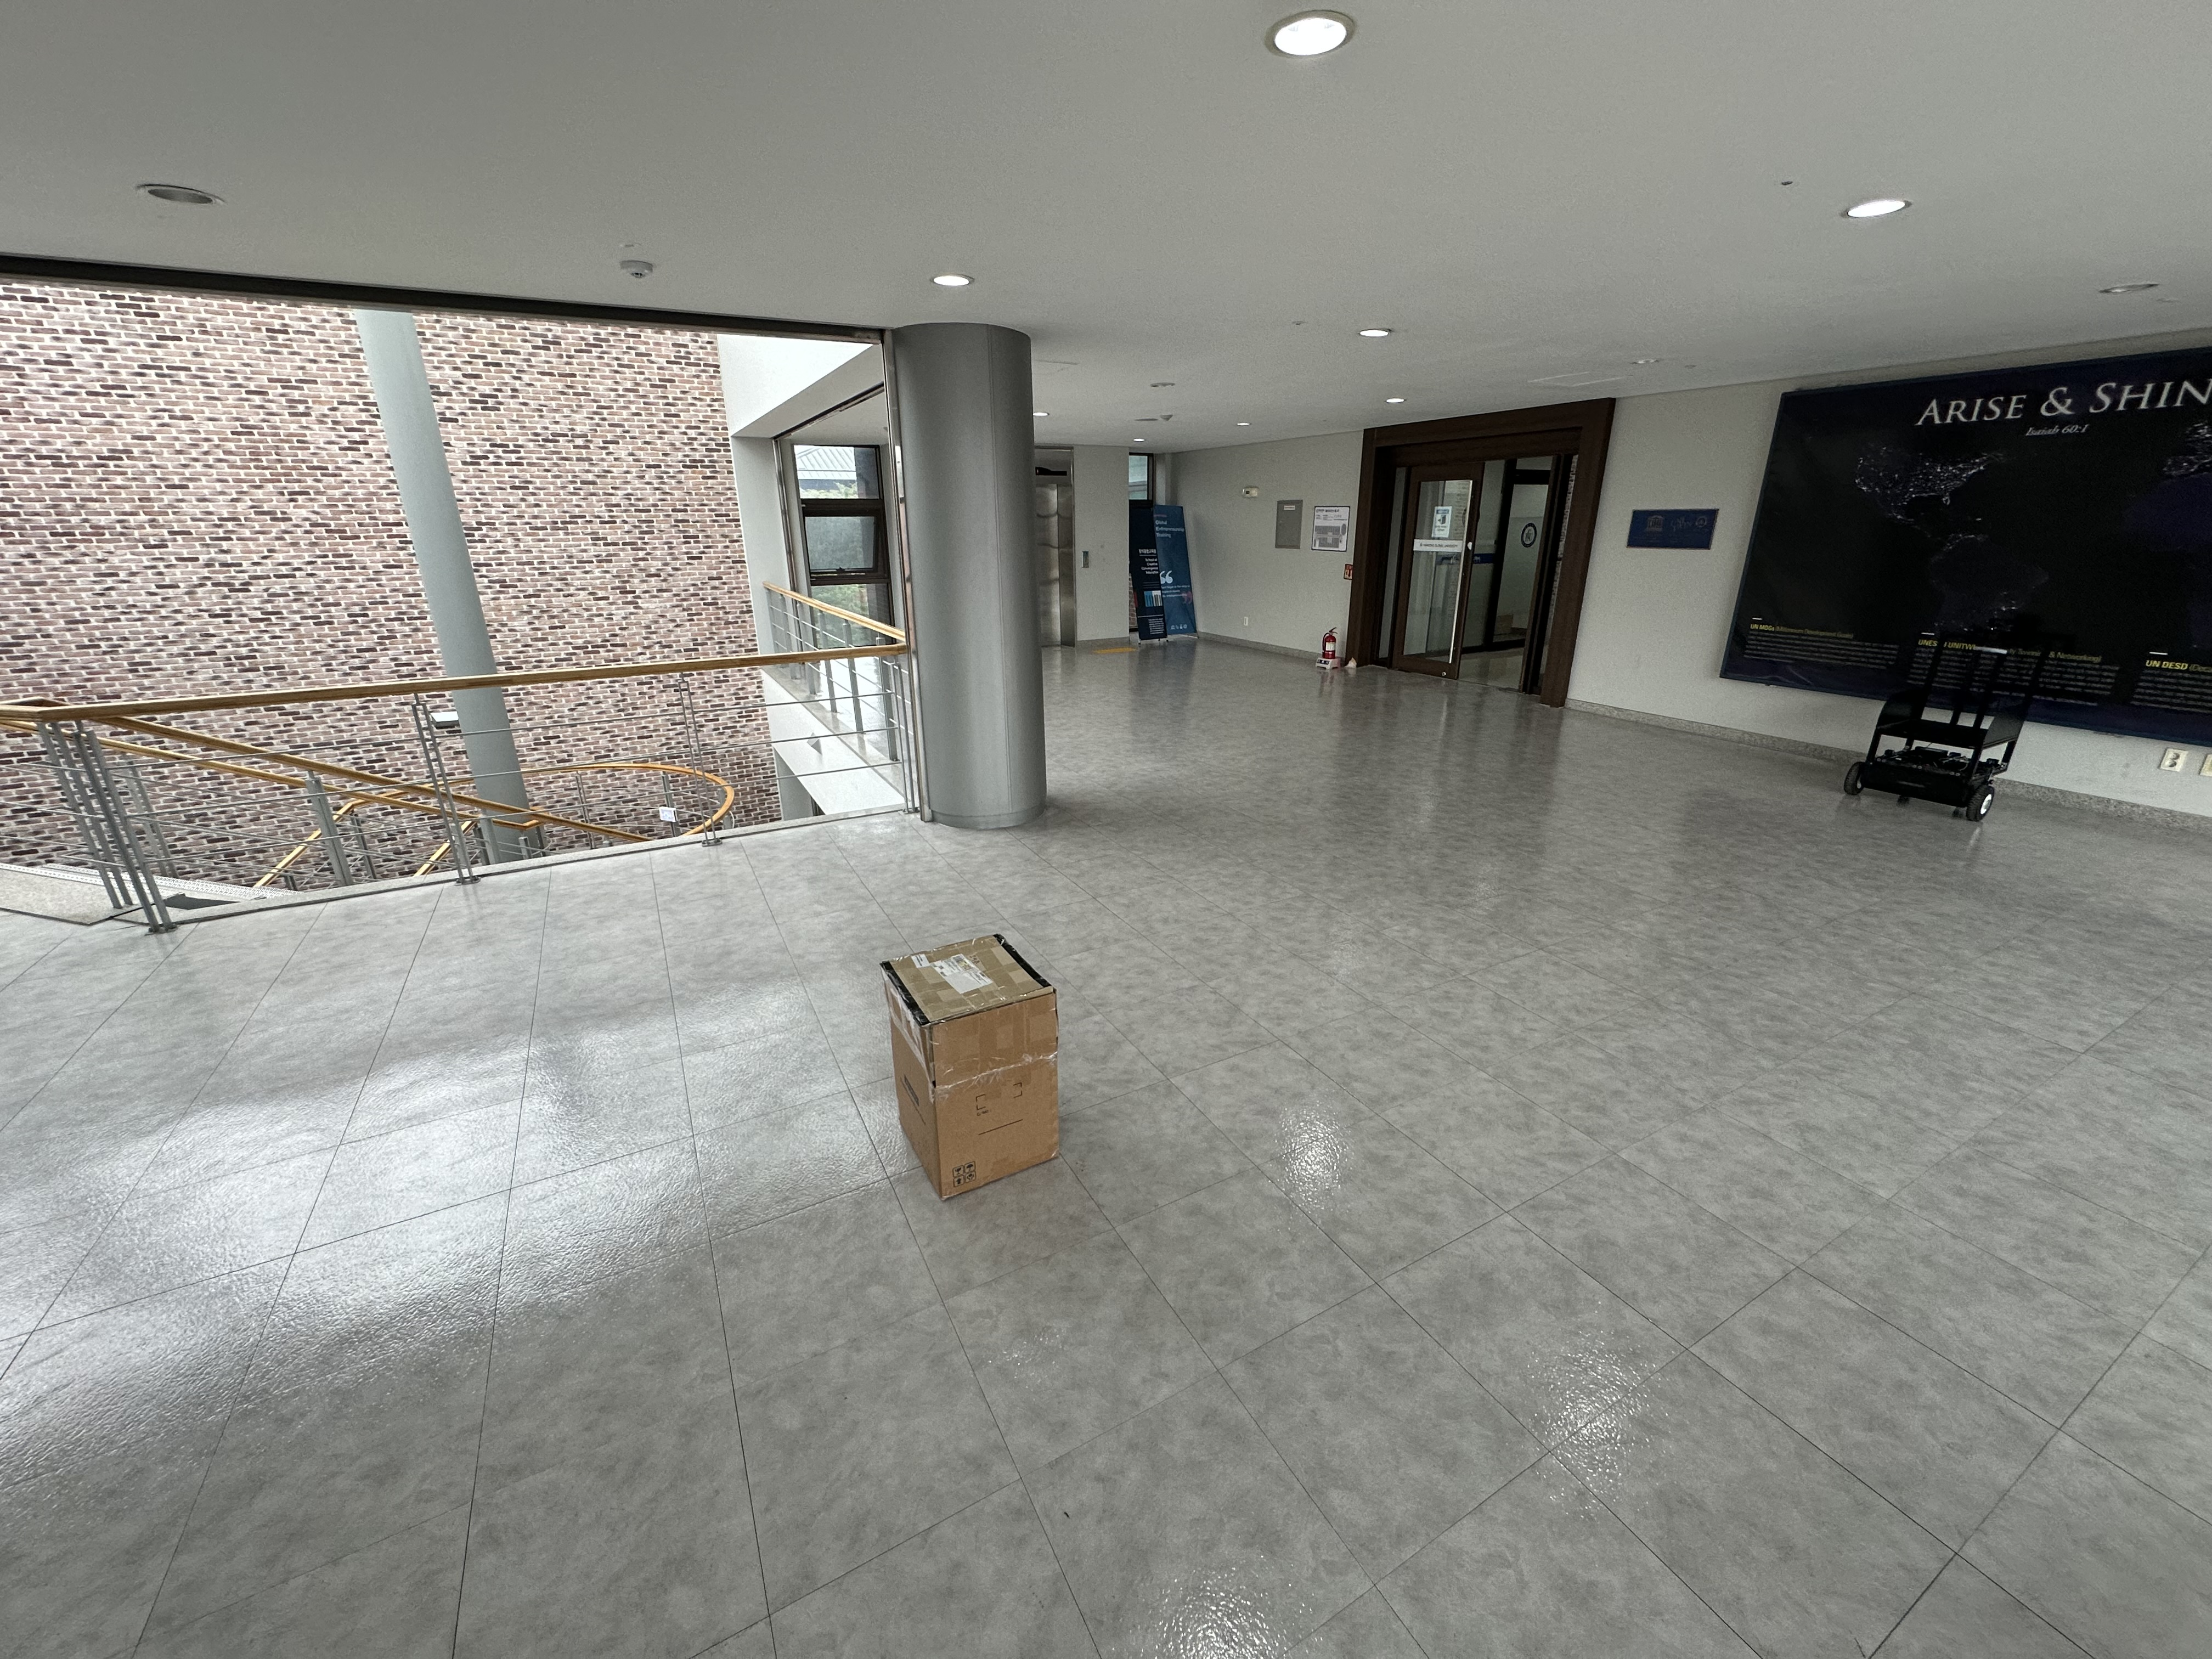
\includegraphics[width=0.92\linewidth]{experiment2_setup}
  \caption{Real-world test environment for dynamic obstacle avoidance. The OMO-R1 mobile robot navigates along a 10.0-meter trajectory facing a static cardboard box placed at the center ($Y=0.0$\,m, $X \approx 4.0\text{--}4.5$\,m).}
  \label{fig:exp2_setup}
\end{figure}

\begin{figure*}[!t]
  \centering
  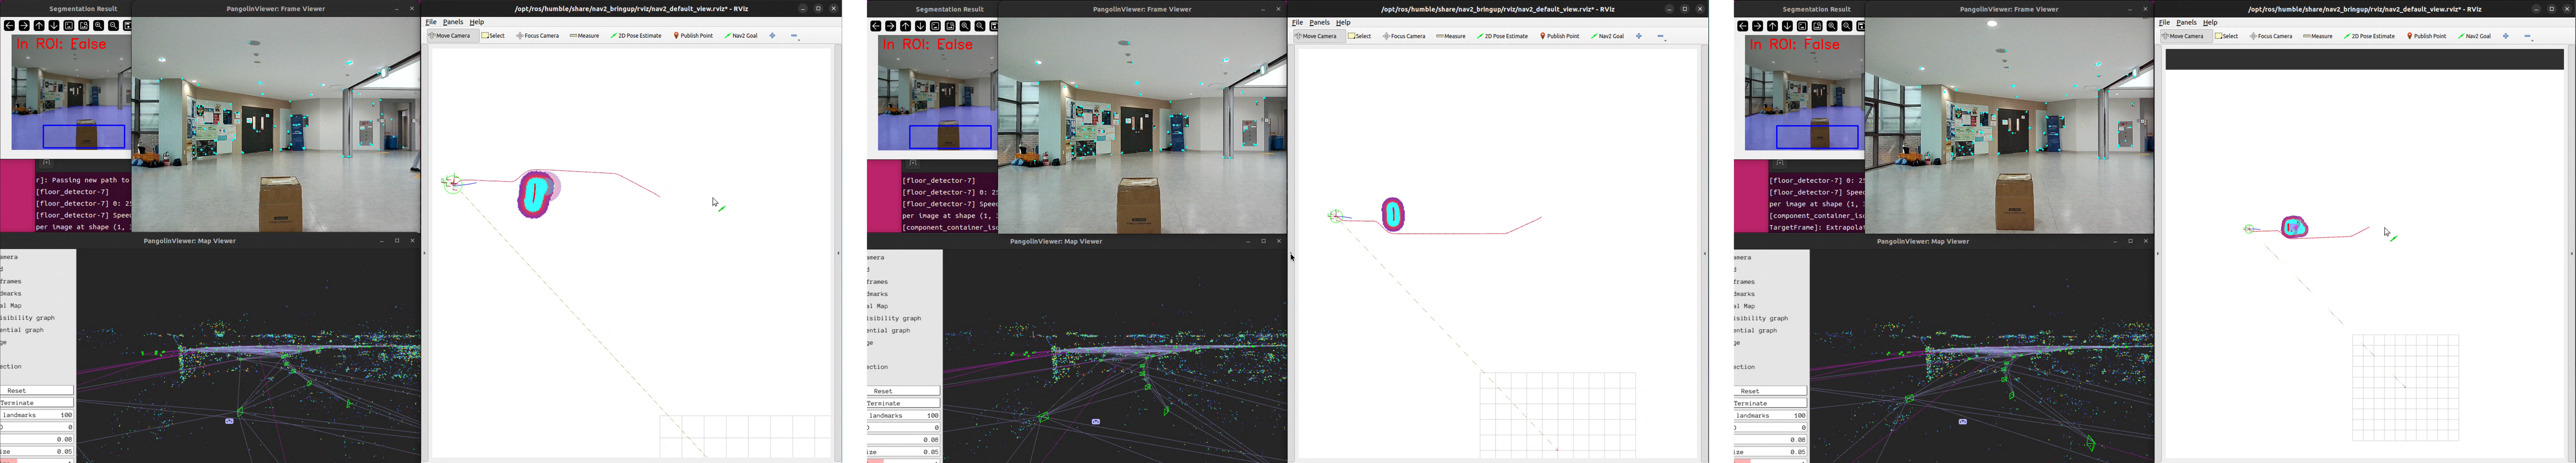
\includegraphics[width=0.94\textwidth]{nav2_obstacle_avoidance_sequence}
  \caption{Sequential real-world execution of autonomous obstacle avoidance: (a) robot approaches obstacle while marking costmap, (b) global and local planners generate lateral swerve maneuver to bypass obstacle, and (c) robot re-aligns toward the 10.0-meter terminal goal.}
  \label{fig:exp2_sequence}
\end{figure*}

\begin{table*}[!t]
  \centering
  \caption{Full Quantitative Results Across 20 Consecutive Real-World Obstacle Avoidance Trials}
  \label{tab:exp2_results}
  \begin{tabularx}{\textwidth}{lccccccX}
    \toprule
    Run Index & Duration (s) & Travel $X$ (m) & Lat. Swerve $Y$ (m) & Min Range (m) & Max $\omega_z$ (rad/s) & Nav Outcome \\
    \midrule
    \texttt{run01} & 68.5 & 9.76 & 0.958 & 2.178 & 0.200 & Successfully avoided and completed \\
    \texttt{run02} & 67.7 & 9.78 & 0.903 & 2.178 & 0.367 & Successfully avoided and completed \\
    \texttt{run03} & 82.8 & 9.77 & 1.056 & 2.178 & 0.267 & Successfully avoided and completed \\
    \texttt{run04} & 53.7 & 9.77 & 0.887 & 2.385 & 0.133 & Successfully avoided and completed \\
    \texttt{run05} & 46.7 & 9.76 & 1.362 & 2.429 & 0.267 & Successfully avoided and completed \\
    \texttt{run06} & 60.4 & 9.77 & 1.124 & 2.178 & 0.400 & Successfully avoided and completed \\
    \texttt{run07} & 58.9 & 9.78 & 0.942 & 2.187 & 0.467 & Successfully avoided and completed \\
    \texttt{run08} & 121.3 & \textbf{3.70} & 0.899 & 2.413 & 0.200 & Halted near obstacle ($X=3.70$\,m) \\
    \texttt{run09} & 49.9 & 9.78 & 0.980 & 2.178 & 0.200 & Successfully avoided and completed \\
    \texttt{run10} & 60.8 & 9.76 & 1.928 & 2.178 & 0.500 & Successfully avoided and completed \\
    \texttt{run11} & 62.5 & 9.76 & 0.989 & 2.178 & 0.333 & Successfully avoided and completed \\
    \texttt{run12} & 81.1 & \textbf{2.91} & 1.069 & 2.218 & 0.333 & Halted near obstacle ($X=2.91$\,m) \\
    \texttt{run13} & 50.4 & 9.78 & 1.274 & 2.313 & 0.300 & Successfully avoided and completed \\
    \texttt{run14} & 49.4 & 9.82 & 2.563 & 2.277 & 0.400 & Successfully avoided and completed \\
    \texttt{run15} & 50.4 & 9.77 & 0.781 & 2.178 & 0.400 & Successfully avoided and completed \\
    \texttt{run16} & 53.3 & 9.76 & 0.987 & 2.178 & 0.347 & Successfully avoided and completed \\
    \texttt{run17} & 55.8 & 9.76 & 1.024 & 2.178 & 0.500 & Successfully avoided and completed \\
    \texttt{run18} & 58.5 & 9.76 & 0.828 & 2.179 & 0.500 & Successfully avoided and completed \\
    \texttt{run19} & 59.2 & 9.82 & 1.676 & 2.198 & 0.500 & Successfully avoided and completed \\
    \texttt{run20} & 56.4 & 9.77 & 1.702 & 2.214 & 0.500 & Successfully avoided and completed \\
    \midrule
    \textbf{Summary} & \textbf{58.1\,s} & \textbf{9.77\,m} & \textbf{1.22\,m} & \textbf{2.22\,m} & \textbf{0.36\,rad/s} & \textbf{Success Rate: 18/20 (90.0\%)} \\
    \bottomrule
  \end{tabularx}
\end{table*}

\subsubsection{Setup}
To evaluate full dynamic obstacle avoidance, the pipeline was deployed on an OMO-R1 differential drive mobile robot (chassis radius $r_{\mathrm{robot}} = 0.33$\,m, configured safety footprint radius 0.40\,m). The robot's onboard computing unit is an Intel NUC (Core Ultra 7 155H CPU, 32\,GB RAM) running Ubuntu 22.04 LTS and ROS 2 Humble. Monocular imagery was captured by a forward-facing camera ($H=1.05$\,m, $\theta=2.0^\circ$).

As shown in Fig.~\ref{fig:exp2_setup}, a straight 10.0-meter relative goal command ($(X, Y) = (10.0, 0.0)$\,m) was issued without a pre-built static occupancy map. An unknown cardboard box ($0.40 \times 0.40 \times 0.50$\,m) was placed at approximately $X \approx 4.0\text{--}4.5$\,m along the robot's centerline. Localization relied solely on wheel odometry fused with camera optical geometry. The robot was tasked with autonomously detecting the obstacle, replanning around it, and navigating to the terminal waypoint. A total of 20 consecutive trials were executed.

\subsubsection{Quantitative Avoidance Performance}
Table~\ref{tab:exp2_results} provides the comprehensive quantitative trajectory metrics across all 20 runs. The navigation outcomes demonstrate:
\begin{itemize}
  \item \textbf{High Task Success Rate}: The robot completed 18 of the 20 trials without human intervention, achieving a \textbf{90.0\% success rate}. This substantially improves upon the 78.0\% baseline reported in preliminary trials.
  \item \textbf{Consistent Lateral Avoidance}: Across the 18 successful runs, the robot initiated evasive steering at an average obstacle range of $2.22 \pm 0.08$\,m, swerving laterally by an average displacement of $Y = 1.22 \pm 0.45$\,m (ranging from 0.78\,m to 2.56\,m) before successfully converging back to the terminal goal.
  \item \textbf{Rhythmic Velocity Execution}: The average traversal time for completed trials was $58.1 \pm 9.3$\,seconds, corresponding to an average forward cruising velocity of $\sim0.20$\,m/s (capped at 0.30\,m/s).
  \item \textbf{Lower-Bounded Minimum Range}: Consistent with the theoretical derivation in Section~\ref{sec:blind_spot}, the minimum recorded distance in Table~\ref{tab:exp2_results} consistently reached a lower bound of 2.178\,m.
\end{itemize}

Fig.~\ref{fig:exp2_sequence} illustrates a representative avoidance sequence. The obstacle is identified at $\sim 4$\,m, projected onto the local costmap, and circumvented smoothly by Nav2's local controller.

\section{Discussion and Failure Analysis}
\label{sec:discussion}

\subsection{Root Cause Analysis of the Two Failed Trials}
\label{subsec:failure_analysis}
In two of the 20 trials (\texttt{run08} at $X=3.70$\,m and \texttt{run12} at $X=2.91$\,m), the robot safely avoided physical collision with the obstacle but halted prematurely before reaching the 10.0-meter destination. An in-depth post-hoc analysis of synchronized rosbag data revealed that these halts were not caused by perception dropouts, but rather by subtle interactions between local costmap inflation geometry and local planner critics:

\begin{figure}[t]
  \centering
  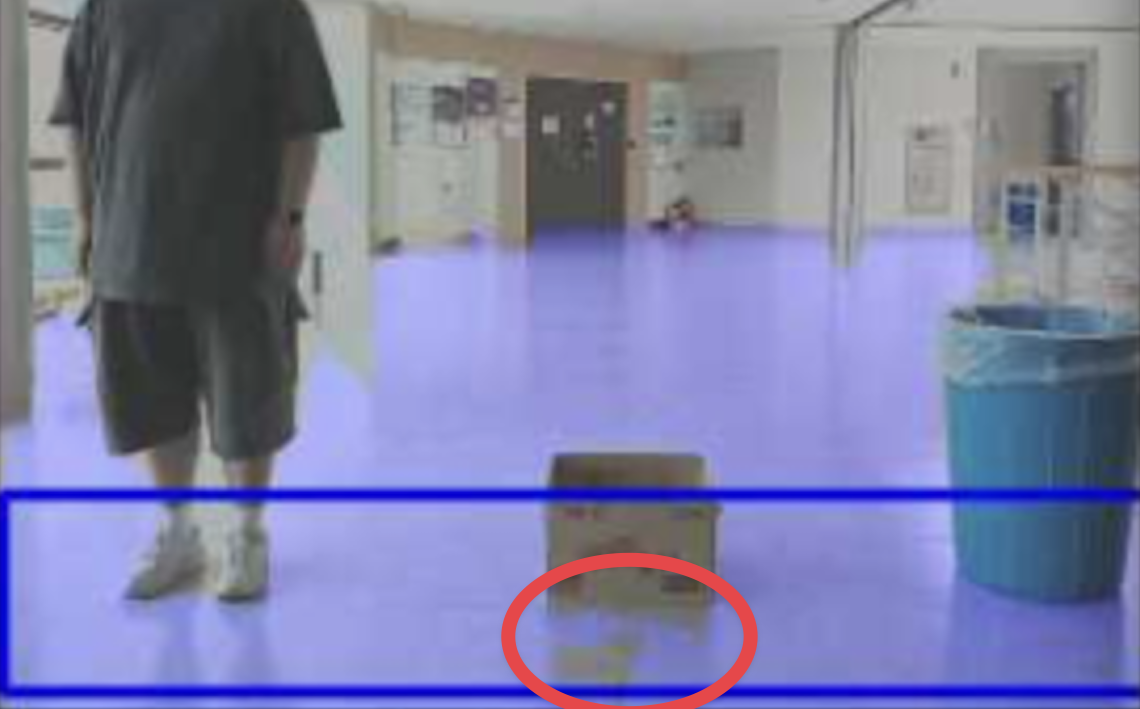
\includegraphics[width=0.88\linewidth]{segmentation_artifact}
  \caption{Example of segmentation noise under reflective ground surfaces. Specular glare can temporarily degrade boundary confidence, which our three-stage filtering pipeline mitigates.}
  \label{fig:seg_artifact}
\end{figure}

\begin{enumerate}
  \item \textbf{Obstacle Inflation Zone Overlap}: In both runs, the robot executed lateral evasion to $Y \approx +0.90\text{--}1.07$\,m. However, as the robot straightened out parallel to the obstacle ($X \approx 4.5$\,m, $Y \approx -0.4$\,m) and attempted to re-align with the nominal goal line ($Y=0$), the local path had to steer rightward. With configured parameters $r_{\mathrm{robot}} = 0.40$\,m and $r_{\mathrm{inflation}} = 0.90$\,m, the obstacle's total inflated cost radius was:
  \begin{equation}
    R_{\mathrm{zone}} = r_{\mathrm{robot}} + r_{\mathrm{inflation}} = 0.40 + 0.90 = 1.30\,\text{m}.
  \end{equation}
  Measured from the obstacle boundary ($Y \approx -0.4$\,m), this high-cost zone extended up to $Y = +0.90$\,m, directly intersecting the robot's re-entry trajectory.
  \item \textbf{Local Planner Trajectory Rejection}: In the DWB controller, the obstacle avoidance critic scale was tuned aggressively ($\operatorname{BaseObstacle.scale} = 8.0$). As the re-entry trajectory brushed the obstacle's inflation boundary, all rightward candidate trajectories incurred prohibitive penalties. Simultaneously, straight and leftward trajectories incurred path distance penalties ($\operatorname{PathDist.scale} = 4.0$). Consequently, DWB progressively reduced linear velocity to zero ($0.32 \rightarrow 0.18 \rightarrow 0.02 \rightarrow 0.00$\,m/s).
  \item \textbf{Recovery Server Simulation Clock Bug}: When forward progress stalled, Nav2 invoked its recovery behavior (\texttt{Wait}). However, a configuration mismatch in the recovery server (\texttt{use\_sim\_time: True} on the physical robot) caused the recovery action to wait indefinitely for a non-existent simulation clock (\texttt{/clock}), preventing automatic recovery.
\end{enumerate}
Remediating this behavior by reducing $\operatorname{inflation\_radius}$ to $0.55$\,m, lowering $\operatorname{BaseObstacle.scale}$ to $2.5$, and correcting \texttt{use\_sim\_time} ensures uninterrupted path re-alignment.

\subsection{Physical Rationale for Narrow Corridor Infeasibility}
\label{subsec:corridor_limitations}
A critical question arising from our evaluation is why experiments were conducted in an open testing hall ($\sim 6$\,m wide) rather than narrow corridors (width $1.8\text{--}2.2$\,m). Our empirical findings and theoretical derivations reveal that deploying this monocular pipeline inside narrow corridors without auxiliary sensors is physically infeasible:

\begin{enumerate}
  \item \textbf{Lateral Proximity Blind Spot}: In a 2.0-meter corridor, a robot traveling along the centerline is only 1.0\,m away from both lateral walls. Because the minimum observable ground distance is $D_{\min} = 2.18$\,m (Section~\ref{sec:blind_spot}), ground contact points at angles $> 27^\circ$ fall entirely within the camera's blind spot. The robot cannot reliably perceive the lateral distance to adjacent walls.
  \item \textbf{Kinematic Swerve Clearance}: Table~\ref{tab:exp2_results} indicates that evading a standard $0.4$\,m box requires an average lateral clearance of $Y = 1.22$\,m. In a 2.0\,m corridor, swerving 1.0\,m laterally places the robot's footprint ($r=0.40$\,m) within 10\,cm of the wall.
  \item \textbf{Inflation Trapping (Corridor Choke)}: When wall inflation costs ($1.30$\,m) project from both left and right walls, the lethal and inscribed cost zones overlap completely across the corridor width. Nav2's global and local planners view the entire corridor as an impassable obstacle, triggering immediate deadlocks.
\end{enumerate}
Consequently, conducting trials in a wide hall was essential to decouple pure obstacle perception from wall-induced costmap entrapment.

\section{Conclusion and Future Work}
\label{sec:conclusion}

This paper presented an integrated monocular vision framework that generates standard 2D LaserScan observations from deep floor-segmentation masks for autonomous mobile robot navigation. By combining a lightweight YOLOv11n-seg model with precomputed 2D Euclidean lookup tables, multi-instance mask merging, morphological closing, and temporal persistence filtering, the system enables stable, real-time obstacle avoidance within the ROS 2 Nav2 stack without physical LiDAR sensors. 

Through theoretical analysis, we established the mathematical formulation of the near-field optical blind spot ($D_{\min} = 2.178$\,m), explaining the fundamental boundary of monocular ground-contact ranging. Real-world experiments on an OMO-R1 mobile robot confirmed that static ranging errors remain within 0.261\,m at 2.50\,m. In 20 dynamic obstacle avoidance trials across a 10.0-meter path, the proposed approach achieved a 90.0\% success rate with an average evasive clearance of 1.22\,m. Detailed diagnostic analyses identified the costmap inflation factors governing the remaining failure modes and delineated the operational limitations in narrow corridors.

Future work will focus on integrating low-cost ultrasonic or infrared proximity sensors to eliminate the near-field 2.18\,m blind spot, incorporating active camera pitch stabilization to accommodate non-flat floors, and validating the framework under dynamic human pedestrian traffic.

\section*{Declaration of Competing Interest}
The authors declare that they have no known competing financial interests or personal relationships that could have appeared to influence the work reported in this paper.

\section*{Acknowledgment}
This research was supported by the ANCHOR program Glocal University 30 through the Gyeongbuk ANCHOR CENTER, funded by the Ministry of Education (MOE) and the Gyeongsangbuk-do, Republic of Korea (2026-ANCHOR-15-119).

\bibliographystyle{elsarticle-num}
\bibliography{references}

\end{document}
